% =====================================================================
%  V2V-Project -- Study Pack
%  Section S6 : The Vehicle Node and TCP Networking
%  Source file studied: node/vehicle_node.py
%  Standalone document -- compile with:  pdflatex 06-vehicle-node-networking.tex
% =====================================================================
\documentclass[11pt,a4paper]{article}

\usepackage[utf8]{inputenc}
\usepackage[T1]{fontenc}
\usepackage{lmodern}

\usepackage[a4paper,margin=2.4cm]{geometry}
\usepackage{enumitem}
\setlist{topsep=2pt,itemsep=2pt}

\usepackage{amsmath}
\usepackage{amssymb}
\usepackage{booktabs}
\usepackage{graphicx}
\usepackage{xcolor}
\usepackage{listings}
\usepackage{tikz}
\usetikzlibrary{arrows.meta,positioning,shapes.geometric,calc,fit,backgrounds}
\usepackage[colorlinks=true,linkcolor=blue,urlcolor=blue,citecolor=blue]{hyperref}

\definecolor{codebg}{rgb}{0.97,0.97,0.94}
\definecolor{codegreen}{rgb}{0.00,0.50,0.00}
\definecolor{codegray}{rgb}{0.50,0.50,0.50}
\definecolor{keyblue}{rgb}{0.00,0.20,0.70}
\definecolor{boxblue}{rgb}{0.88,0.93,1.00}
\definecolor{boxyellow}{rgb}{1.00,0.97,0.85}

\lstdefinestyle{py}{
  language=Python,
  backgroundcolor=\color{codebg},
  basicstyle=\ttfamily\footnotesize,
  keywordstyle=\color{keyblue}\bfseries,
  stringstyle=\color{codegreen},
  commentstyle=\color{codegray}\itshape,
  numberstyle=\tiny\color{codegray},
  numbers=left,
  numbersep=8pt,
  showstringspaces=false,
  breaklines=true,
  breakatwhitespace=false,
  frame=single,
  rulecolor=\color{codegray},
  tabsize=4,
  captionpos=b,
}
\lstdefinestyle{term}{
  backgroundcolor=\color{codebg},
  basicstyle=\ttfamily\footnotesize,
  breaklines=true,
  frame=single,
  rulecolor=\color{codegray},
  numbers=none,
  captionpos=b,
}

\title{\textbf{V2V-Project Study Pack}\\[4pt]
       \large Section S6 --- The Vehicle Node and TCP Networking}
\author{Information Security Project --- Beginner Study Notes}
\date{Source file: \texttt{node/vehicle\_node.py}}

\begin{document}
\maketitle
\tableofcontents
\newpage

% =====================================================================
\section{Title and ``What You'll Learn''}
% =====================================================================

\subsection*{Section Title}
\textbf{S6 --- The Vehicle Node: the program you actually run, which connects two
cars over a real network and drives the whole security pipeline end to end.}

\subsection*{Plain-English Summary (read this first)}
Everything so far --- certificates, crypto, the handshake, the message protocol
--- has been a \emph{library}. Section~S6 is the \textbf{program}. One file,
\texttt{vehicle\_node.py}, is launched once per car. One car acts as the
\textbf{server} (it waits for a connection); the other acts as the
\textbf{client} (it dials in). They make a real network connection using
\textbf{TCP}, run the 4-step handshake over it, and then continuously send and
receive encrypted safety messages --- one per second --- using background
\textbf{threads}. S6 is the conductor that calls S2, S3, S4 and S5 in the right
order.

\subsection*{Learning Outcomes}
After studying this section you will be able to:
\begin{itemize}
  \item Explain what \textbf{TCP} and a \textbf{socket} are.
  \item Explain the \textbf{message-framing} problem and how a 4-byte length
        header solves it.
  \item Explain the difference between the \textbf{server} and \textbf{client}
        roles.
  \item Explain why \textbf{threads} are needed and what a \emph{daemon} thread is.
  \item Explain \textbf{connection retries} with exponential backoff.
  \item Walk through every function and method of \texttt{vehicle\_node.py}.
  \item Launch two vehicle nodes, read their logs, and explain how the receive
        loop reacts to an attack.
\end{itemize}

% =====================================================================
\section{Where This Fits}
% =====================================================================

S6 is not one stage of the pipeline --- it is the \emph{frame around all three
stages}. It loads the identity files from S2, builds the \texttt{AuthProtocol}
of S4 (which rests on the crypto of S3), runs the handshake, and then repeatedly
calls the \texttt{secure\_send} / \texttt{secure\_receive} of S5. It also starts
the dashboard of S7. In short: S6 is the integration layer.

\begin{center}
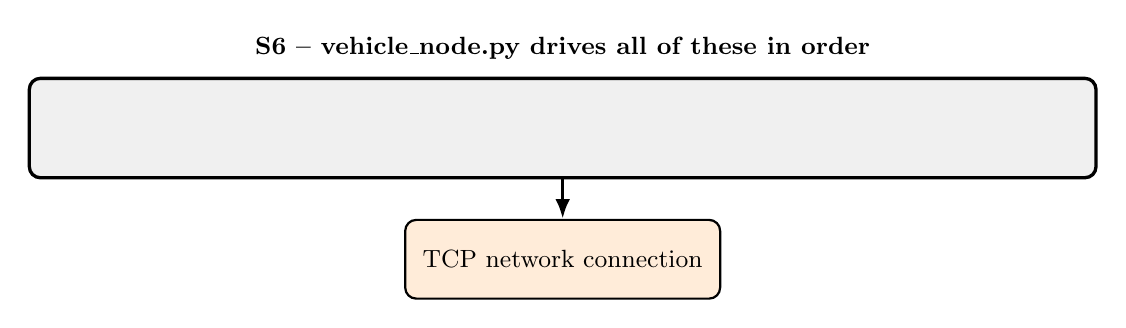
\begin{tikzpicture}[font=\small,node distance=6mm and 8mm,
   st/.style={draw,rounded corners,minimum width=2.7cm,minimum height=1.0cm,
              align=center,thick}]
  \node[st,fill=boxblue]   (id)   {Identity\\\scriptsize S2};
  \node[st,fill=red!12,right=of id]   (cr) {Crypto\\\scriptsize S3};
  \node[st,fill=green!12,right=of cr] (au) {Handshake\\\scriptsize S4};
  \node[st,fill=boxyellow,right=of au] (ms) {Messaging\\\scriptsize S5};
  \node[draw,very thick,rounded corners,fill=gray!12,fit=(id)(cr)(au)(ms)] (box) {};
  \node[above=1mm of box,font=\small\bfseries] {S6 -- vehicle\_node.py drives all of these in order};
  \node[below=5mm of box,st,fill=orange!15,minimum width=4cm] (net) {TCP network connection};
  \draw[-{Latex[length=2.5mm]},very thick] (box) -- (net);
\end{tikzpicture}
\end{center}

% =====================================================================
\section{The Theory You Must Study}
% =====================================================================

\subsection{TCP and Sockets}
\textbf{Plain definition.} \textbf{TCP} (Transmission Control Protocol) is a way
for two programs to send data to each other reliably and in order across a
network. A \textbf{socket} is the software ``end point'' of a connection --- the
object a program reads from and writes to, like the handset of a telephone.

\textbf{Real-life analogy.} A telephone call. TCP is the phone system that makes
sure your words arrive, in order, with nothing dropped. The socket is the handset
in your hand.

\textbf{Why it exists.} The two vehicles run as separate programs (possibly on
separate laptops). They need a dependable channel: TCP guarantees that bytes
arrive complete and in the order they were sent --- something a raw network does
not promise.

\textbf{How it works here.} The code uses Python's \texttt{socket} module.
\texttt{socket.socket(AF\_INET, SOCK\_STREAM)} creates a TCP socket. The server
\emph{binds} to a port and \emph{listens}; the client \emph{connects}.

\textbf{Security property it provides.} None. \textbf{This is important:} TCP is
\emph{not} encrypted. The radio/network is still untrusted. All the security
comes from the \emph{payload} (the SecureBSM of S5), not from TCP.

\subsection{The Message-Framing Problem}
\textbf{Plain definition.} TCP delivers a \emph{byte stream} --- an unbroken flow
of bytes with \emph{no markers} showing where one message ends and the next
begins. \emph{Framing} is the technique of adding those markers.

\textbf{Real-life analogy.} Imagine a friend reading you a long list of phone
numbers with no pauses: ``07700900461077009005...''. Without a gap or a stated
length, you cannot tell where one number ends. Framing is agreeing in advance:
``each number is exactly 11 digits''.

\textbf{Why it exists.} A single \texttt{recv()} call might return half a message,
or two messages stuck together. Without framing the receiver cannot reliably
split the stream into messages.

\textbf{How it works here.} The project uses \textbf{length-prefix framing}.
Before every message, \texttt{send\_framed} writes a 4-byte big-endian number
saying how long the message is. \texttt{recv\_framed} first reads exactly those
4 bytes, learns the length, then reads exactly that many more bytes.

\textbf{Security property it provides.} None directly --- but reliable framing
prevents parsing confusion that an attacker might otherwise exploit.

\subsection{Server and Client Roles}
\textbf{Plain definition.} The \textbf{server} is the side that waits to be
contacted (it \emph{listens} on a port). The \textbf{client} is the side that
starts the conversation (it \emph{connects} to the server's address).

\textbf{Real-life analogy.} A shop and a customer. The shop opens its doors and
waits (server). The customer walks in (client). After that, both can talk freely.

\textbf{Why it exists.} \emph{Someone} has to be reachable first. One side must
be ready and waiting before the other can connect.

\textbf{How it works here.} A vehicle started \emph{without} \texttt{--peer-host}
is a pure server: it just waits. A vehicle started \emph{with}
\texttt{--peer-host} also starts its own server thread \emph{and} then connects
to the peer as a client. In the handshake, the client becomes the
\emph{initiator} (sends HELLO first) and the server becomes the
\emph{responder}.

\textbf{Security property it provides.} None --- it is about connection setup.

\subsection{Threads and Concurrency}
\textbf{Plain definition.} A \textbf{thread} is a separate line of execution
inside the same program, so the program can do more than one thing at a time.

\textbf{Real-life analogy.} One person can only talk \emph{or} listen at once. To
have a real conversation you need two people: one always ready to speak, one
always ready to listen. Threads give the program that second ``person''.

\textbf{Why it exists.} Sending a BSM every second and receiving BSMs at any time
must happen \emph{simultaneously}. If the program were stuck waiting to receive,
it could never send, and vice versa. So the node runs a \emph{send loop} in one
thread and a \emph{receive loop} in another.

\textbf{How it works here.} \texttt{threading.Thread(target=..., daemon=True)}
creates a thread. A \textbf{daemon} thread is one that does not keep the program
alive on its own --- when the main program exits, daemon threads stop too. The
node uses daemon threads for the server-accept loop, the send loop, the receive
loop and the dashboard.

\textbf{Security property it provides.} None --- it is about doing two jobs at once.

\subsection{Connection Retries and Exponential Backoff}
\textbf{Plain definition.} If the client cannot connect (the server is not ready
yet), it tries again. \emph{Exponential backoff} means waiting a bit longer
before each retry.

\textbf{Real-life analogy.} Phoning a friend who is busy: you call, wait a
minute, call again, wait two minutes, call again --- you do not redial
non-stop.

\textbf{Why it exists.} When two laptops start at slightly different times, the
client may dial before the server is listening. Retrying with growing pauses
gives the server time to come up without hammering the network.

\textbf{How it works here.} \texttt{connect\_to\_peer} tries up to five times; on
failure it sleeps \texttt{2 * attempt} seconds (2\,s, 4\,s, 6\,s, 8\,s) before
the next try.

\textbf{Security property it provides.} None --- it is about robustness.

% =====================================================================
\section{Code Walkthrough}
% =====================================================================

\subsection{The TCP framing helpers}
\begin{lstlisting}[style=py,caption={vehicle\_node.py --- length-prefix framing helpers.}]
def send_framed(sock: socket.socket, data: bytes) -> None:
    """Send *data* prefixed with a 4-byte length header."""
    sock.sendall(struct.pack(">I", len(data)) + data)

def _recv_exactly(sock: socket.socket, n: int) -> bytes:
    """Block until exactly *n* bytes have been received."""
    buf = b""
    while len(buf) < n:
        chunk = sock.recv(n - len(buf))
        if not chunk:
            raise ConnectionError("Connection closed by peer")
        buf += chunk
    return buf

def recv_framed(sock: socket.socket) -> bytes:
    """Receive a length-prefixed message."""
    header = _recv_exactly(sock, 4)
    length = struct.unpack(">I", header)[0]
    return _recv_exactly(sock, length)
\end{lstlisting}
\textbf{Step by step:}
\begin{enumerate}
  \item \texttt{send\_framed}: \texttt{struct.pack(">I", len(data))} makes a
        4-byte big-endian length; it is glued in front of \texttt{data};
        \texttt{sock.sendall} sends the whole thing.
  \item \texttt{\_recv\_exactly}: a single \texttt{recv} may return fewer bytes
        than asked, so this loops, collecting \texttt{chunk}s, until it has
        exactly \texttt{n} bytes. If \texttt{recv} returns nothing, the peer hung
        up --- it raises \texttt{ConnectionError}.
  \item \texttt{recv\_framed}: read exactly 4 bytes (the header), decode the
        length, then read exactly that many more bytes --- one complete message.
\end{enumerate}
\textbf{Theory link:} solves the message-framing problem. \emph{Analogy:} each
parcel has its weight on the label, so you know when you have it all.

\subsection{VehicleNode.\_\_init\_\_ --- set the node up}
\textbf{Purpose:} load the identity files, build the protocol objects, create the
server socket.
\begin{lstlisting}[style=py,caption={vehicle\_node.py --- the VehicleNode constructor (key parts).}]
class VehicleNode:
    def __init__(self, vehicle_id, port, cert_path, key_path, ca_cert_path,
                 bsm_interval=1.0, dashboard_port=5000):
        # Load cryptographic material
        self.cert_pem = Path(cert_path).read_bytes()
        self.private_key = load_private_key(Path(key_path).read_bytes())
        self.ca_cert_pem = Path(ca_cert_path).read_bytes()
        # Build the AuthProtocol instance (S4)
        self.auth = AuthProtocol(vehicle_id, self.private_key,
                                 self.cert_pem, self.ca_cert_pem)
        # Message subsystem (S5)
        self.logger = MessageLogger()
        self.replay_cache = ReplayCache()
        self.timestamp_validator = TimestampValidator(max_age_seconds=5.0)
        # Session state -- filled in after the handshake
        self.session_key = None
        self.peer_public_key = None
        # Networking
        self.server_sock = socket.socket(socket.AF_INET, socket.SOCK_STREAM)
        self.server_sock.setsockopt(socket.SOL_SOCKET, socket.SO_REUSEADDR, 1)
        self.running = True
        self._seq = 0
        self._last_peer_seq = None
\end{lstlisting}
\textbf{Step by step:}
\begin{enumerate}
  \item Read the vehicle's certificate, private key and the CA certificate from
        disk (the S2 artifacts).
  \item Build an \texttt{AuthProtocol} object --- the S4 handshake engine.
  \item Create the S5 messaging helpers: a \texttt{MessageLogger}, a
        \texttt{ReplayCache} and a \texttt{TimestampValidator}.
  \item Prepare empty session slots --- \texttt{session\_key} and
        \texttt{peer\_public\_key} stay \texttt{None} until the handshake
        completes.
  \item Create a TCP server socket. \texttt{SO\_REUSEADDR} lets the program
        re-bind the same port quickly after a restart instead of waiting for the
        operating system to release it.
  \item \texttt{\_seq} counts outgoing BSMs; \texttt{\_last\_peer\_seq} remembers
        the last sequence number received (for the S5 replay check).
\end{enumerate}
\textbf{Theory link:} this constructor wires S2 + S3 + S4 + S5 together.

\subsection{start\_server() and \_accept\_loop() --- the server role}
\begin{lstlisting}[style=py,caption={vehicle\_node.py --- listening for a peer.}]
def start_server(self) -> None:
    self.server_sock.bind(("0.0.0.0", self.port))
    self.server_sock.listen(1)
    t = threading.Thread(target=self._accept_loop, daemon=True)
    t.start()

def _accept_loop(self) -> None:
    conn, addr = self.server_sock.accept()        # blocks until a peer connects
    self._run_handshake_responder(conn)
\end{lstlisting}
\textbf{Step by step:}
\begin{enumerate}
  \item \texttt{bind(("0.0.0.0", port))} attaches the socket to the chosen port
        on every network interface (\texttt{0.0.0.0} = ``all addresses'').
  \item \texttt{listen(1)} marks it ready to accept one queued connection.
  \item The actual waiting happens in a \emph{daemon thread} so the main program
        is not frozen.
  \item \texttt{accept()} blocks until a peer connects, then hands the new
        connection to the \emph{responder} handshake.
\end{enumerate}
\textbf{Theory link:} the server role; threads. \emph{Analogy:} the shop opening
its doors and a staff member waiting at the entrance.

\subsection{connect\_to\_peer() --- the client role with retries}
\begin{lstlisting}[style=py,caption={vehicle\_node.py --- connecting to a peer, with backoff.}]
def connect_to_peer(self, host, port) -> bool:
    retries = 5
    for attempt in range(1, retries + 1):
        try:
            conn = socket.socket(socket.AF_INET, socket.SOCK_STREAM)
            conn.settimeout(10)
            conn.connect((host, port))
            conn.settimeout(None)
            self._run_handshake_initiator(conn)
            return True
        except (ConnectionRefusedError, OSError) as exc:
            if attempt < retries:
                time.sleep(2 * attempt)        # exponential backoff
    return False
\end{lstlisting}
\textbf{Step by step:}
\begin{enumerate}
  \item Try up to five times.
  \item Create a fresh socket; \texttt{settimeout(10)} means ``give up a single
        connect attempt after 10 seconds''.
  \item \texttt{connect((host, port))} dials the peer. On success,
        \texttt{settimeout(None)} switches back to normal blocking mode and the
        \emph{initiator} handshake runs.
  \item On failure, sleep \texttt{2 * attempt} seconds (growing each time) and
        retry. After five failures, give up and return \texttt{False}.
\end{enumerate}
\textbf{Theory link:} the client role; exponential backoff.

\subsection{The two handshake drivers}
\begin{lstlisting}[style=py,caption={vehicle\_node.py --- driving the 4-step handshake over the socket.}]
def _run_handshake_initiator(self, conn):
    hello = self.auth.build_hello()                       # Step 1
    send_framed(conn, hello.to_json().encode())
    challenge = ChallengeMessage.from_json(recv_framed(conn).decode())  # Step 2
    response = self.auth.process_challenge(challenge)      # Step 3
    send_framed(conn, response.to_json().encode())
    ack = AckMessage.from_json(recv_framed(conn).decode()) # Step 4
    self.session_key = self.auth.process_ack(ack)
    self.peer_public_key = self.auth.peer_public_key
    self._start_comm_threads(conn)

def _run_handshake_responder(self, conn):
    hello = HelloMessage.from_json(recv_framed(conn).decode())          # Step 1
    challenge = self.auth.process_hello(hello)             # Step 2
    send_framed(conn, challenge.to_json().encode())
    response = ResponseMessage.from_json(recv_framed(conn).decode())    # Step 3
    ack = self.auth.process_response(response, hello)      # Step 4
    send_framed(conn, ack.to_json().encode())
    self.session_key = self.auth.session_key
    self._start_comm_threads(conn)
\end{lstlisting}
\textbf{Step by step:} these two methods take the abstract S4 handshake and run
it over the real socket.
\begin{enumerate}
  \item The \emph{initiator} builds and sends HELLO, receives CHALLENGE, sends
        RESPONSE, receives ACK --- calling the S4 \texttt{AuthProtocol} methods
        and using \texttt{to\_json}/\texttt{from\_json} to turn each message into
        bytes and back.
  \item The \emph{responder} mirrors it: receive HELLO, send CHALLENGE, receive
        RESPONSE, send ACK.
  \item Both end by storing \texttt{session\_key} and \texttt{peer\_public\_key},
        then calling \texttt{\_start\_comm\_threads}.
  \item If any step raises \texttt{AuthError}, the handshake is abandoned and the
        connection closed --- no session, no messaging.
\end{enumerate}
\textbf{Theory link:} this is S4 made real over a network. \emph{Analogy:} the
secret handshake actually performed at the door, not just rehearsed.

\subsection{The send and receive loops}
\begin{lstlisting}[style=py,caption={vehicle\_node.py --- the two BSM loops (one per thread).}]
def _start_comm_threads(self, conn):
    threading.Thread(target=self._bsm_send_loop, args=(conn,), daemon=True).start()
    threading.Thread(target=self._receive_loop, args=(conn,), daemon=True).start()

def _bsm_send_loop(self, conn):
    while self.running:
        self._seq += 1
        bsm = BasicSafetyMessage(vehicle_id=self.vehicle_id,
            speed_kmh=round(random.uniform(60, 100), 1), heading_deg=45.0,
            latitude=6.9271 + random.uniform(-0.001, 0.001),
            longitude=79.8612 + random.uniform(-0.001, 0.001),
            timestamp=time.time(), sequence_num=self._seq,
            brake_applied=random.random() < 0.1,
            acceleration=round(random.uniform(-2, 3), 1))
        wire = secure_send(bsm, self.session_key, self.private_key, self.logger)
        send_framed(conn, wire)
        time.sleep(self.bsm_interval)

def _receive_loop(self, conn):
    while self.running:
        try:
            raw = recv_framed(conn)
            bsm = secure_receive(raw, self.session_key, self.peer_public_key,
                self.replay_cache, self.timestamp_validator, self.logger,
                last_seq=self._last_peer_seq)
            self._last_peer_seq = bsm.sequence_num
        except TamperError as exc:
            log.warning("[%s] TAMPER ALERT: %s", self.vehicle_id, exc)
        except (ReplayError, SequenceError) as exc:
            log.warning("[%s] REPLAY ALERT: %s", self.vehicle_id, exc)
        except ConnectionError:
            break
\end{lstlisting}
\textbf{Step by step:}
\begin{enumerate}
  \item \texttt{\_start\_comm\_threads} launches \emph{two} daemon threads so
        sending and receiving run at the same time.
  \item \textbf{Send loop:} every \texttt{bsm\_interval} seconds (default 1),
        increment the sequence counter, build a BSM with slightly-randomised
        values, call \texttt{secure\_send} (S5) to sign+encrypt it, then
        \texttt{send\_framed} it.
  \item \textbf{Receive loop:} read one framed message, call
        \texttt{secure\_receive} (S5) to decrypt and verify it, and remember its
        sequence number.
  \item \textbf{The security reaction:} if \texttt{secure\_receive} raises
        \texttt{TamperError}, the loop logs a \emph{TAMPER ALERT} and
        \emph{keeps running} --- it does not crash. \texttt{ReplayError} /
        \texttt{SequenceError} give a \emph{REPLAY ALERT}. A real
        \texttt{ConnectionError} ends the loop.
\end{enumerate}
\textbf{Theory link:} threads (two loops at once); this is where S5's exceptions
become visible security events. \emph{Analogy:} a guard who, on spotting a fake,
notes it in the logbook and carries on watching --- rather than fainting.

\subsection{get\_state() and shutdown()}
\texttt{get\_state} gathers a snapshot --- certificate status, authentication
status, peer id, recent messages, alerts and counters --- as a dictionary for the
S7 dashboard to display. \texttt{shutdown} sets \texttt{running = False} (so the
loops stop) and closes the server socket.

\subsection{main() --- the program entry point}
\texttt{main} reads the command-line arguments (\texttt{--vehicle-id},
\texttt{--port}, \texttt{--cert}, \texttt{--key}, \texttt{--ca-cert},
optional \texttt{--peer-host}/\texttt{--peer-port}, \texttt{--dashboard-port}),
builds the \texttt{VehicleNode}, starts the Flask dashboard in a daemon thread,
starts the TCP server, and --- if a \texttt{--peer-host} was given --- connects
as a client. It then keeps the main thread alive until \texttt{Ctrl+C}.

% =====================================================================
\section{Hands-On / Practical}
% =====================================================================

\subsection{Run two vehicle nodes}
You need the certificates first (Section~S2). Then open \emph{two} PowerShell
terminals.

\textbf{Terminal 1 --- Vehicle A (server):}
\begin{lstlisting}[style=term]
python node\vehicle_node.py --vehicle-id vehicle-a --port 9001 `
  --cert ca\certs\vehicle-a_cert.pem --key ca\certs\vehicle-a_key.pem `
  --ca-cert ca\certs\ca_cert.pem --dashboard-port 5001
\end{lstlisting}

\textbf{Terminal 2 --- Vehicle B (client):}
\begin{lstlisting}[style=term]
python node\vehicle_node.py --vehicle-id vehicle-b --port 9002 `
  --cert ca\certs\vehicle-b_cert.pem --key ca\certs\vehicle-b_key.pem `
  --ca-cert ca\certs\ca_cert.pem --peer-host 127.0.0.1 --peer-port 9001 `
  --dashboard-port 5002
\end{lstlisting}

\noindent\textbf{Expected output (sample, Vehicle B):}
\begin{lstlisting}[style=term]
[10:00:01] INFO: [vehicle-b] Listening on port 9002 ...
[10:00:01] INFO: [vehicle-b] Dashboard at http://localhost:5002
[10:00:02] INFO: [vehicle-b] Connecting to 127.0.0.1:9001 (attempt 1/5)...
[10:00:02] INFO: [vehicle-b] === AUTHENTICATED with vehicle-a ===
[10:00:03] INFO: [vehicle-b] BSM #1 sent: speed=82.4 km/h
[10:00:03] INFO: [vehicle-b] BSM #1 from vehicle-a: speed=77.1 km/h VERIFIED
[10:00:04] INFO: [vehicle-b] BSM #2 sent: speed=69.8 km/h
[10:00:04] INFO: [vehicle-b] BSM #2 from vehicle-a: speed=91.3 km/h VERIFIED
\end{lstlisting}

\subsection{What the output lines mean}
\begin{itemize}
  \item \texttt{Listening on port 9002} --- the server thread is up.
  \item \texttt{Connecting ... (attempt 1/5)} --- the client role dialling A.
  \item \texttt{=== AUTHENTICATED with vehicle-a ===} --- the 4-step handshake
        succeeded; a session key now exists.
  \item \texttt{BSM \#1 sent} --- the send loop fired once (one second later).
  \item \texttt{BSM \#1 from vehicle-a ... VERIFIED} --- the receive loop got a
        BSM and \texttt{secure\_receive} passed every check.
\end{itemize}

\subsection{Try This Yourself (mini-experiment)}
Start Vehicle~B \emph{first}, before Vehicle~A exists.\\
\textbf{Predict before you run.} B's server starts, then B tries to connect to A.
A is not there, so \texttt{connect\_to\_peer} fails attempt~1 and sleeps 2~s,
fails attempt~2 and sleeps 4~s, and so on --- you should see
\texttt{(attempt 1/5)}, \texttt{(attempt 2/5)} ... with growing pauses. Now start
Vehicle~A within those ~20 seconds: the next retry \emph{succeeds} and the
handshake runs. This demonstrates exponential backoff making startup order not
matter.

% =====================================================================
\section{Attack Relevance}
% =====================================================================

S6 does not invent a new defence --- it is the layer that \emph{deploys} every
earlier defence and makes the system react to attacks at runtime.

\begin{table}[h]
\centering
\small
\begin{tabular}{@{}p{2.7cm} p{5.8cm} p{5.0cm}@{}}
\toprule
\textbf{Attack} & \textbf{S6's role in stopping it} & \textbf{Where}\\
\midrule
Tamper & The receive loop catches the \texttt{TamperError} from
\texttt{secure\_receive} and logs a TAMPER ALERT --- without crashing. &
\texttt{\_receive\_loop}.\\
Replay & The receive loop catches \texttt{SequenceError} /
\texttt{ReplayError} and logs a REPLAY ALERT. & \texttt{\_receive\_loop}.\\
MITM / impersonation & A failed handshake raises \texttt{AuthError}; the driver
closes the connection so no session is formed. & \texttt{\_run\_handshake\_*}.\\
Stream desync & Length-prefix framing means a manipulated stream cannot quietly
shift message boundaries. & \texttt{recv\_framed}.\\
\bottomrule
\end{tabular}
\caption{S6 turns the library defences into a running, attack-resistant program.}
\end{table}

\noindent\textbf{The key behaviour:} the receive loop wraps
\texttt{secure\_receive} in \texttt{try/except}. A tampered or replayed BSM
raises an exception, which the loop \emph{catches}, \emph{logs as an alert}, and
then \emph{continues}. An attacker therefore cannot crash a vehicle by feeding it
bad messages --- the node simply rejects them and keeps going.

\textbf{Honest scope note.} S6 carries the security in the \emph{payload}, but
the TCP connection itself is plain. An attacker on the network can still see
\emph{that} two cars are talking, how often, and packet sizes (this is
\emph{metadata}). They cannot read or forge the contents, but the project does
not hide traffic patterns. Also, the server does \texttt{listen(1)} and
\texttt{\_accept\_loop} handles exactly \emph{one} peer --- this is a two-car
simulation, not a scalable many-vehicle network.

% =====================================================================
\section{Illustrations}
% =====================================================================

\subsection{Diagram 1 --- the two-node network}
\begin{center}
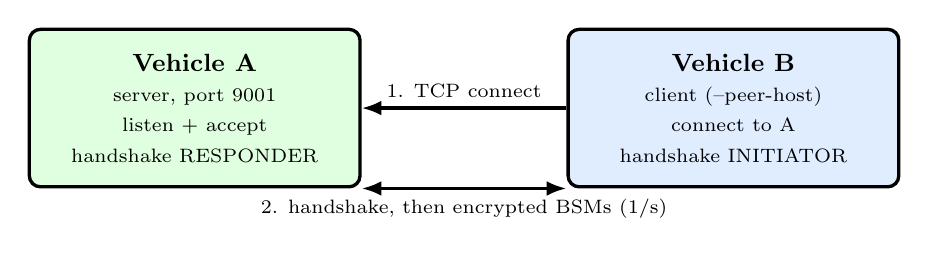
\begin{tikzpicture}[font=\small,node distance=8mm,
   v/.style={draw,very thick,rounded corners,minimum width=4.2cm,minimum height=2.0cm,
             align=center}]
  \node[v,fill=green!12] (a)
       {\textbf{Vehicle A}\\\scriptsize server, port 9001\\
        \scriptsize listen + accept\\\scriptsize handshake RESPONDER};
  \node[v,fill=boxblue,right=26mm of a] (b)
       {\textbf{Vehicle B}\\\scriptsize client (--peer-host)\\
        \scriptsize connect to A\\\scriptsize handshake INITIATOR};
  \draw[-{Latex[length=2.5mm]},very thick] (b) -- (a)
       node[midway,above,font=\scriptsize]{1. TCP connect};
  \draw[{Latex[length=2.5mm]}-{Latex[length=2.5mm]},very thick] (a.south east) -- (b.south west)
       node[midway,below,font=\scriptsize]{2. handshake, then encrypted BSMs (1/s)};
\end{tikzpicture}
\end{center}

\subsection{Diagram 2 --- length-prefix framing}
\begin{center}
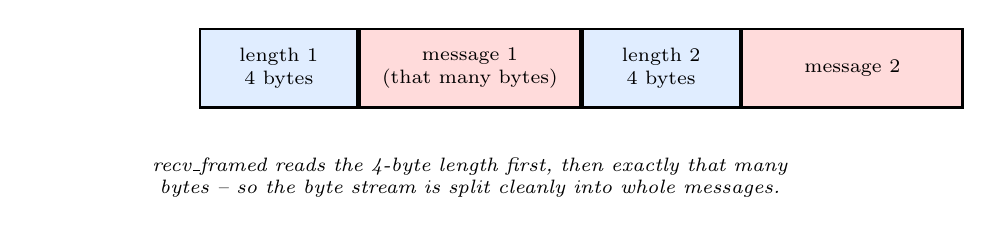
\begin{tikzpicture}[font=\scriptsize,node distance=4mm,
   f/.style={draw,thick,minimum height=1.0cm,align=center}]
  \node[f,fill=boxblue,minimum width=2.0cm] (h1) {length 1\\4 bytes};
  \node[f,fill=red!14,minimum width=2.8cm,right=0 of h1] (m1) {message 1\\(that many bytes)};
  \node[f,fill=boxblue,minimum width=2.0cm,right=0 of m1] (h2) {length 2\\4 bytes};
  \node[f,fill=red!14,minimum width=2.8cm,right=0 of h2] (m2) {message 2};
  \node[below=5mm of m1,font=\scriptsize\itshape,text width=11cm,align=center]
       {recv\_framed reads the 4-byte length first, then exactly that many bytes
        -- so the byte stream is split cleanly into whole messages.};
\end{tikzpicture}
\end{center}

\subsection{Diagram 3 --- the two communication threads}
\begin{center}
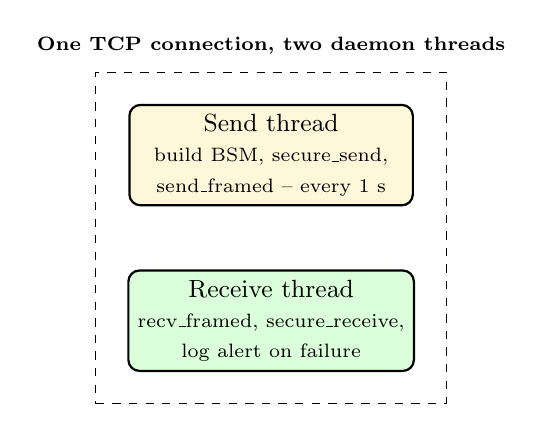
\begin{tikzpicture}[font=\small,node distance=7mm,
   t/.style={draw,thick,rounded corners,minimum width=3.6cm,minimum height=1.2cm,
             align=center}]
  \node[t,fill=boxyellow] (snd) {Send thread\\\scriptsize build BSM, secure\_send,\\\scriptsize send\_framed -- every 1 s};
  \node[t,fill=green!14,below=8mm of snd] (rcv) {Receive thread\\\scriptsize recv\_framed, secure\_receive,\\\scriptsize log alert on failure};
  \node[draw,dashed,fit=(snd)(rcv),inner sep=4mm] (box) {};
  \node[above=1mm of box,font=\scriptsize\bfseries] {One TCP connection, two daemon threads};
\end{tikzpicture}
\end{center}

% =====================================================================
\section{Presentation Pack}
% =====================================================================

\subsection{Slide Outline}

\textbf{Slide 1 --- From Library to Program.}
\begin{itemize}
  \item S2--S5 were libraries; S6 is the program you run.
  \item One file, \texttt{vehicle\_node.py}, launched once per car.
  \item It loads identity, runs the handshake, exchanges BSMs.
  \item It also starts the monitoring dashboard.
\end{itemize}

\textbf{Slide 2 --- TCP, Sockets and Framing.}
\begin{itemize}
  \item TCP = a reliable, ordered byte stream between two programs.
  \item But a stream has no message boundaries.
  \item Fix: a 4-byte length header before every message.
  \item \texttt{recv\_framed} reads the length, then exactly that many bytes.
\end{itemize}

\textbf{Slide 3 --- Server, Client and the Handshake.}
\begin{itemize}
  \item One car listens (server); the other connects (client).
  \item Client connects with up to 5 retries and exponential backoff.
  \item Client = handshake initiator; server = responder.
  \item A failed handshake (\texttt{AuthError}) $\to$ connection closed.
\end{itemize}

\textbf{Slide 4 --- Two Threads: Send and Receive.}
\begin{itemize}
  \item Sending and receiving must happen at the same time.
  \item Send thread: one encrypted BSM every second.
  \item Receive thread: decrypt + verify every incoming BSM.
  \item Both are daemon threads --- they stop when the program stops.
\end{itemize}

\textbf{Slide 5 --- Reacting to Attacks at Runtime.}
\begin{itemize}
  \item The receive loop wraps \texttt{secure\_receive} in try/except.
  \item \texttt{TamperError} $\to$ TAMPER ALERT, logged, keep running.
  \item \texttt{SequenceError} $\to$ REPLAY ALERT, logged, keep running.
  \item An attacker cannot crash the node with bad messages.
\end{itemize}

\subsection{Speaker Talking Points (about 30--60 seconds each)}

\textbf{Slide 1.} ``Everything we have built so far has been a library --- code
that other code calls. Section six is different: it is the actual program. You
launch vehicle\_node.py once for each car. It loads that car's certificate and
keys, opens a network connection to the other car, runs the four-step handshake,
and then settles into exchanging encrypted safety messages once a second. It even
starts the web dashboard. So this file is the conductor that brings sections two
through five together into one running system.''

\textbf{Slide 2.} ``The cars talk over TCP. TCP is like a reliable phone line ---
bytes arrive complete and in order. But TCP has one quirk: it delivers an
unbroken stream of bytes with no markers showing where one message stops and the
next starts. Imagine someone reading phone numbers aloud with no pauses. Our fix
is framing: before every message we write a four-byte number saying how long the
message is. The receiver reads those four bytes first, learns the length, then
reads exactly that many bytes --- one clean message, every time.''

\textbf{Slide 3.} ``Someone has to be reachable first, so one car is the server:
it opens a port and waits. The other is the client: it dials in. Because the two
laptops may start at different times, the client retries up to five times, and
waits a little longer before each retry --- two seconds, four, six --- so-called
exponential backoff. Once connected, the client plays the initiator in the
handshake and the server plays the responder. If the handshake fails --- a bad
certificate or a bad signature --- the code raises an AuthError and simply closes
the connection. No session, no messaging.''

\textbf{Slide 4.} ``A real conversation needs you to speak and listen at the same
time. A single line of code can only do one thing at once, so the node uses two
threads. The send thread builds a safety message, secures it, and sends it ---
once every second, forever. The receive thread waits for incoming messages,
decrypts and verifies each one. They run side by side. Both are daemon threads,
which just means they shut down automatically when the main program exits.''

\textbf{Slide 5.} ``Here is the security behaviour that matters at runtime. The
receive loop calls secure\_receive inside a try/except block. If a message has
been tampered with, secure\_receive throws a TamperError --- the loop catches it,
writes a TAMPER ALERT to the log, and carries on. A replayed message throws a
SequenceError and becomes a REPLAY ALERT. The node never crashes. So an attacker
flooding it with bad messages just fills the alert log --- they cannot take the
vehicle down.''

\subsection{Live-Demo Script}
\begin{enumerate}
  \item \textbf{Open two terminals.} Start Vehicle~A (server), then Vehicle~B
        (client) with the commands above.
  \item \textbf{Point at the handshake line.} \texttt{=== AUTHENTICATED with
        vehicle-a ===} --- ``the four-step handshake just ran over the network.''
  \item \textbf{Point at the BSM lines.} \texttt{BSM \#n sent} and \texttt{BSM
        \#n ... VERIFIED} --- ``send thread and receive thread, both running.''
  \item \textbf{Show robustness.} Mention that running an attack script against
        the node produces a TAMPER/REPLAY ALERT line but the node keeps going.
  \item \textbf{Optional.} Start B before A to show the retry/backoff messages.
\end{enumerate}

\subsection{Examiner Q\&A}
\begin{enumerate}
  \item \textbf{Q: What is TCP, and does it provide security here?}\\
        A: TCP is a reliable, ordered byte-stream protocol between two programs.
        It provides \emph{no} security --- the connection is plain. All security
        is in the SecureBSM payload (S5).
  \item \textbf{Q: What is the framing problem and how is it solved?}\\
        A: TCP gives a boundary-less byte stream. The fix is a 4-byte big-endian
        length header before each message; \texttt{recv\_framed} reads the length
        then exactly that many bytes.
  \item \textbf{Q: Why does \texttt{\_recv\_exactly} use a loop?}\\
        A: A single \texttt{recv} may return fewer bytes than requested, so the
        loop keeps reading until exactly \texttt{n} bytes are collected.
  \item \textbf{Q: What is the difference between the server and client?}\\
        A: The server binds a port and waits (\texttt{listen}/\texttt{accept});
        the client connects to the server's address. The client is the handshake
        initiator, the server the responder.
  \item \textbf{Q: Why are two threads needed?}\\
        A: Sending a BSM every second and receiving BSMs must happen
        simultaneously; one thread runs the send loop, the other the receive
        loop. Daemon threads stop automatically when the program exits.
  \item \textbf{Q: What is exponential backoff and why use it?}\\
        A: Waiting longer before each retry (2\,s, 4\,s, 6\,s...). It lets a
        slow-starting server come up without the client hammering the network.
  \item \textbf{Q: What happens when a tampered BSM arrives?}\\
        A: \texttt{secure\_receive} raises \texttt{TamperError}; the receive loop
        catches it, logs a TAMPER ALERT, and continues --- the node does not crash.
  \item \textbf{Q: Name a limitation of this networking design.}\\
        A: The server accepts exactly one peer (\texttt{listen(1)}), so it is a
        two-car simulation, not a scalable network. Also, traffic metadata
        (timing, sizes, the fact that two cars talk) is visible even though
        contents are protected.
\end{enumerate}

% =====================================================================
\section{Glossary}
% =====================================================================
\begin{description}[style=nextline,leftmargin=0pt]
  \item[TCP] Transmission Control Protocol: reliable, ordered byte-stream networking.
  \item[Socket] The software end point of a network connection.
  \item[Byte stream] A continuous flow of bytes with no message boundaries.
  \item[Framing] Adding markers so a stream can be split into messages.
  \item[Length-prefix] A length number written just before a message.
  \item[Big-endian] Byte order with the most significant byte first.
  \item[Server] The side that listens and waits to be contacted.
  \item[Client] The side that initiates the connection.
  \item[bind / listen / accept] Server socket steps: claim a port, mark ready, take a connection.
  \item[connect] The client socket step: dial the server.
  \item[Port] A numbered endpoint on a computer that a program listens behind.
  \item[0.0.0.0] ``All network interfaces'' --- bind on every local address.
  \item[SO\_REUSEADDR] A socket option allowing quick re-binding of a port after restart.
  \item[Thread] A separate line of execution inside one program.
  \item[Daemon thread] A thread that does not keep the program alive on its own.
  \item[Concurrency] Doing more than one task in overlapping time.
  \item[Exponential backoff] Waiting progressively longer before each retry.
  \item[Initiator / Responder] The two handshake roles (client / server here).
  \item[VehicleNode] The class representing one running vehicle.
  \item[secure\_send / secure\_receive] The S5 functions the loops call.
  \item[TamperError / SequenceError] Exceptions the receive loop catches and logs.
  \item[Metadata] Information about traffic (timing, size) rather than its content.
\end{description}

% =====================================================================
\section{References and Further Study}
% =====================================================================
\begin{itemize}
  \item \textbf{Python socket module documentation} ---
        \url{https://docs.python.org/3/library/socket.html}\\
        Read for: \texttt{bind}, \texttt{listen}, \texttt{accept},
        \texttt{connect}, \texttt{recv}, \texttt{sendall}.
  \item \textbf{Python socket programming HOWTO} ---
        \url{https://docs.python.org/3/howto/sockets.html}\\
        Read for: a beginner walk-through of client/server sockets and framing.
  \item \textbf{Python threading module documentation} ---
        \url{https://docs.python.org/3/library/threading.html}\\
        Read for: \texttt{Thread}, daemon threads, concurrency.
  \item \textbf{Transmission Control Protocol (Wikipedia)} ---
        \url{https://en.wikipedia.org/wiki/Transmission_Control_Protocol}\\
        Read for: what TCP guarantees and how it works.
  \item \textbf{Network socket (Wikipedia)} ---
        \url{https://en.wikipedia.org/wiki/Network_socket}\\
        Read for: the socket concept explained simply.
  \item \textbf{Exponential backoff (Wikipedia)} ---
        \url{https://en.wikipedia.org/wiki/Exponential_backoff}\\
        Read for: why retry delays grow.
  \item \textbf{Python struct module documentation} ---
        \url{https://docs.python.org/3/library/struct.html}\\
        Read for: the 4-byte big-endian length header (\texttt{">I"}).
  \item \textbf{Python argparse documentation} ---
        \url{https://docs.python.org/3/library/argparse.html}\\
        Read for: how the command-line options are parsed in \texttt{main}.
  \item \textbf{Beej's Guide to Network Programming} ---
        \url{https://beej.us/guide/bgnet/}\\
        Read for: a famous, friendly introduction to sockets and framing.
\end{itemize}

\vfill
\begin{center}\footnotesize\itshape
End of Section S6. Next: S7 --- the Flask monitoring dashboard that visualises
this running node.
\end{center}

\end{document}
